\documentclass[10pt,mathserif]{beamer}

\usepackage{graphicx,amsmath,amssymb}
\usepackage{subcaption, natbib, hyperref}
\hypersetup{
    colorlinks=true,
    linkcolor=blue,
    filecolor=magenta,
    urlcolor=cyan,
}

% ------------------------------------------------------------------------
% Packages
% ------------------------------------------------------------------------
\usepackage{amsmath}

% ------------------------------------------------------------------------
% Macros
% ------------------------------------------------------------------------
%~~~~~~~~~~~~~~~
% List shorthand
%~~~~~~~~~~~~~~~
\newcommand{\BIT}{\begin{itemize}}
\newcommand{\EIT}{\end{itemize}}
\newcommand{\BNUM}{\begin{enumerate}}
\newcommand{\ENUM}{\end{enumerate}}
%~~~~~~~~~~~~~~~
% Text with quads around it
%~~~~~~~~~~~~~~~
\newcommand{\qtext}[1]{\quad\text{#1}\quad}
%~~~~~~~~~~~~~~~
% Shorthand for math formatting
%~~~~~~~~~~~~~~~
\newcommand\mbb[1]{\mathbb{#1}}
\newcommand\mbf[1]{\mathbf{#1}}
\def\mc#1{\mathcal{#1}}
\def\mrm#1{\mathrm{#1}}
%~~~~~~~~~~~~~~~
% Common sets
%~~~~~~~~~~~~~~~
\def\reals{\mathbb{R}} % Real number symbol
\def\integers{\mathbb{Z}} % Integer symbol
\def\rationals{\mathbb{Q}} % Rational numbers
\def\naturals{\mathbb{N}} % Natural numbers
\def\complex{\mathbb{C}} % Complex numbers
\def\simplex{\mathcal{S}} % Simplex
%~~~~~~~~~~~~~~~
% Common functions
%~~~~~~~~~~~~~~~
\renewcommand{\exp}[1]{\operatorname{exp}\left(#1\right)} % Exponential
\def\indic#1{\mbb{I}\left({#1}\right)} % Indicator function
\providecommand{\argmax}{\mathop\mathrm{arg max}} % Defining math symbols
\providecommand{\argmin}{\mathop\mathrm{arg min}}
\providecommand{\arccos}{\mathop\mathrm{arccos}}
\providecommand{\asinh}{\mathop\mathrm{asinh}}
\providecommand{\dom}{\mathop\mathrm{dom}} % Domain
\providecommand{\range}{\mathop\mathrm{range}} % Range
\providecommand{\diag}{\mathop\mathrm{diag}}
\providecommand{\tr}{\mathop\mathrm{tr}}
\providecommand{\abs}{\mathop\mathrm{abs}}
\providecommand{\card}{\mathop\mathrm{card}}
\providecommand{\sign}{\mathop\mathrm{sign}}
\def\rank#1{\mathrm{rank}({#1})}
\def\supp#1{\mathrm{supp}({#1})}
%~~~~~~~~~~~~~~~
% Common probability symbols
%~~~~~~~~~~~~~~~
\def\E{\mathbb{E}} % Expectation symbol
\def\Earg#1{\E\left[{#1}\right]}
\def\Esubarg#1#2{\E_{#1}\left[{#2}\right]}
\def\P{\mathbb{P}} % Probability symbol
\def\Parg#1{\P\left({#1}\right)}
\def\Psubarg#1#2{\P_{#1}\left[{#2}\right]}
\def\Cov{\mrm{Cov}} % Covariance symbol
\def\Covarg#1{\Cov\left[{#1}\right]}
\def\Covsubarg#1#2{\Cov_{#1}\left[{#2}\right]}
\def\Var{\mrm{Var}}
\def\Vararg#1{\Var\left(#1\right)}
\def\Varsubarg#1#2{\Var_{#1}\left(#2\right)}
\newcommand{\family}{\mathcal{P}} % probability family
\newcommand{\eps}{\epsilon}
\def\absarg#1{\left|#1\right|}
\def\msarg#1{\left(#1\right)^{2}}
\def\logarg#1{\log\left(#1\right)}
%~~~~~~~~~~~~~~~
% Distributions
%~~~~~~~~~~~~~~~
\def\Gsn{\mathcal{N}}
\def\Ber{\textnormal{Ber}}
\def\Bin{\textnormal{Bin}}
\def\Unif{\textnormal{Unif}}
\def\Mult{\textnormal{Mult}}
\def\Cat{\textnormal{Cat}}
\def\Gam{\textnormal{Gam}}
\def\InvGam{\textnormal{InvGam}}
\def\NegMult{\textnormal{NegMult}}
\def\Dir{\textnormal{Dir}}
\def\Lap{\textnormal{Laplace}}
\def\Bet{\textnormal{Beta}}
\def\Poi{\textnormal{Poi}}
\def\HypGeo{\textnormal{HypGeo}}
\def\GEM{\textnormal{GEM}}
\def\BP{\textnormal{BP}}
\def\DP{\textnormal{DP}}
\def\BeP{\textnormal{BeP}}
%~~~~~~~~~~~~~~~
% Theorem-like environments
%~~~~~~~~~~~~~~~

%-----------------------
% Probability sets
%-----------------------
\newcommand{\X}{\mathcal{X}}
\newcommand{\Y}{\mathcal{Y}}
\newcommand{\D}{\mathcal{D}}
\newcommand{\Scal}{\mathcal{S}}
%-----------------------
% vector notation
%-----------------------
\newcommand{\bx}{\mathbf{x}}
\newcommand{\by}{\mathbf{y}}
\newcommand{\bt}{\mathbf{t}}
\newcommand{\xbar}{\overline{x}}
\newcommand{\Xbar}{\overline{X}}
\newcommand{\tolaw}{\xrightarrow{\mathcal{L}}}
\newcommand{\toprob}{\xrightarrow{\mathbb{P}}}
\newcommand{\laweq}{\overset{\mathcal{L}}{=}}
\newcommand{\F}{\mathcal{F}}
\def\colarg#1#2{\textcolor[HTML]{#1}{#2}}


\mode<presentation>
{
\usetheme{default}
}
\setbeamertemplate{navigation symbols}{}
\usecolortheme[rgb={0.13,0.28,0.59}]{structure}
\setbeamertemplate{itemize subitem}{--}
\setbeamertemplate{frametitle} {
	\begin{center}
	  {\large\bf \insertframetitle}
	\end{center}
}

\AtBeginSection[]
{
	\begin{frame}<beamer>
		\frametitle{Outline}
		\tableofcontents[currentsection,currentsubsection]
	\end{frame}
}

%% begin presentation

\title{\large \bfseries Technology for Good\\ Perspectives from Bangalore
  and Chicago}

\author{Kris Sankaran\\[3ex]}

\date{\today}

\begin{document}
\maketitle

\begin{frame}
  \frametitle{We are not the first!}
  \begin{itemize}
  \item We should learn the most effective strategies from past projects (in AI
    or adjacent domains)
  \item In this talk, focus on two
    \begin{itemize}
    \item ICTD: Internet Communication Technology for Development, especially as
      developed at Microsoft Research Bangalore
    \item DSSG: Data Science for Social Good, at the University of Chicago
    \end{itemize}
  \item Perspectives are quite different, but I think we can learn from both
  \end{itemize}
\end{frame}

\section{Chicago}
\label{sec:chicago}
\subsection{Examples}

\begin{frame}
  \frametitle{Adverse Interactions}
  \begin{itemize}
  \item Examples: Unjustified use of force, sustained citizen or officer
    complaints, unjustified searches, ...
  \item Partnered with Charolette-Mecklenburg Police
  \item Already had state-of-the art Early Intervention System
    \begin{itemize}
    \item But just manually defined decision rules
    \end{itemize}
  \end{itemize}
\begin{figure}[ht]
  \centering
  \includegraphics[width=0.5\paperwidth]{figures/eis}
  \caption{The original EIS interface.\label{fig:label} }
\end{figure}

\end{frame}

\begin{frame}
  \frametitle{Recipe}
  \begin{itemize}
  \item Formulation as ML problems
  \item Flag at-risk officers, with enough lead-time to provide intervention
  \item Flag at-risk dispatches, and try to send best-suited officers
  \end{itemize}
  \begin{figure}[ht]
    \centering
    \includegraphics[width=0.35\paperwidth]{figures/adverse_flagged}
    \caption{\label{fig:label} Example at risk officers. Color is feature importance. }
  \end{figure}
\end{frame}

\begin{frame}
  \frametitle{Recipe}
  \begin{itemize}
  \item Collect all sorts of potentially relevant data
  \end{itemize}
  \begin{figure}
    \centering
    \includegraphics[width=0.8\paperwidth]{figures/adverse_data_source}
    \caption{Sources of data going into ML system. \label{fig:label} }
\end{figure}
\end{frame}

\begin{frame}
  \frametitle{Recipe}
  \begin{itemize}
  \item Handcraft all sorts of potentially useful features
    \begin{itemize}
    \item Officer characteristics
    \item Situational factors
    \item Neighborhood factors
    \end{itemize}
  \end{itemize}
  \begin{figure}[ht]
    \centering
    \includegraphics[width=0.6\paperwidth]{figures/adverse_features}
    \caption{Examples of important features. \label{fig:label} }
  \end{figure}
\end{frame}

\begin{frame}
  \frametitle{Subtleties}
  \begin{itemize}
  \item Implementation issues
    \begin{itemize}
    \item Which interventions to take?
    \item How effective are they for different subgroups?
    \end{itemize}
  \item Puzzle: Want interpretability, but don't want to risk gameability
  \end{itemize}
\end{frame}

\begin{frame}
  \frametitle{High School Dropout}
  \begin{itemize}
  \item Identify students at risk of dropout before it's to late to do anything
    about it
  \item Partnered with two large school districts
    \begin{itemize}
    \item 200,000 students
    \item $\sim 5 - 10\%$ dropout rates
    \end{itemize}
  \end{itemize}
  \begin{figure}
    \centering
    \includegraphics[width=0.7\paperwidth]{figures/academic_paper}
  \end{figure}
\end{frame}

\begin{frame}
  \frametitle{Recipe}
  \begin{itemize}
  \item ML Formulation: Precision and recall at the $k$-students who you have
    the resources to intervent on
  \item Temporal cross-validation
  \end{itemize}
  \begin{figure}[ht]
    \centering
    \includegraphics[width=0.6\paperwidth]{figures/precision_curves_academic}
    \caption{Example precision curves for one district. Which model you choose
      might depend on how many students you have resources to intervene
      on.\label{fig:label} }
  \end{figure}
\end{frame}

\begin{frame}
  \frametitle{Recipe}
  \begin{itemize}
  \item Collect all sorts of relevant data
  \item Feature engineering + off-the-shelf methods
  \end{itemize}
  \begin{figure}
    \includegraphics[width=0.45\paperwidth]{figures/academic_features_1}
    \includegraphics[width=0.25\paperwidth]{figures/academic_features_2}
    \caption{Example features used for prediction.}
\end{figure}

\end{frame}

\begin{frame}
  \frametitle{Interpretability and Fairness}
  \begin{itemize}
  \item Relied on feature importance for interpretation
  \item Fairness: The \textit{frequent-itemset trick}
    \begin{itemize}
    \item Find frequent itemsets
    \item Compute error rates on each
    \item Characterize subgroups where model is particularly inaccurate
    \end{itemize}
  \item Still have questions about intervention effectiveness
  \end{itemize}
\begin{figure}[ht]
  \centering
  \includegraphics[width=0.7\paperwidth]{figures/freq_items}
  \caption{Types of items that are prone to mistakes. \label{fig:label} }
\end{figure}

\end{frame}

\begin{frame}
  \frametitle{Prioritized Lead Inspection}
  \begin{itemize}
  \item There are lots of negative consequences of infants ingesting lead
  \item Lead paint was banned in 1970, but impossible to remediate all homes
  \item Standard approach: inspect home after positive test result
    \begin{itemize}
    \item Not as crazy as it might seem
    \item Prediction would be nice, but false positives come at cost of
      remediation
    \end{itemize}
  \end{itemize}
\begin{figure}
  \centering
  \includegraphics[width=0.5\paperwidth]{figures/lead_quote}
  \caption{My favorite quote from the paper.}
\end{figure}

\end{frame}

\begin{frame}
  \frametitle{Recipe}
  \begin{itemize}
  \item 2.5 million blood tests from 1993 - 2013
    \begin{itemize}
    \item Manual regexes to fix data entry errors
    \end{itemize}
  \item 120,000 home lead inspection records (more regexes)
  \item Mix in all sorts of public data
  \end{itemize}
  \begin{figure}[ht]
    \centering
    \includegraphics[width=0.5\paperwidth]{figures/lead_data}
    \caption{Sources of data in the lead prediction project.\label{fig:label} }
\end{figure}

\end{frame}

\begin{frame}
  \frametitle{Recipe}
  \begin{itemize}
  \item Handcraft features
    \begin{itemize}
    \item About child
    \item About location
    \item About location-time window
    \end{itemize}
  \item Evaluate using temporal CV
  \end{itemize}
  \begin{figure}[ht]
    \centering
    \includegraphics[width=0.5\paperwidth]{figures/lead_features}
    \caption{Example relevant hand-crafted features.\label{fig:label} }
\end{figure}
\end{frame}

%% \begin{frame}
%%   \frametitle{Interventions}
%%   \begin{itemize}
%%   \item Encourage testing via well-placed billboards
%%   \item Share scores with doctors
%%   \item Send scores to landlords
%%   \end{itemize}
%% \end{frame}

\subsection{Perspectives}

\begin{frame}
  \frametitle{Abstractions}
  \begin{itemize}
  \item Can I detect who's going to get lead poisoning early?
  \item Can I determine which home inspections to prioritize?
  \item Which policies do I modify to improve maternal mortality?
  \item How much impact is my after school program having?
  \item Can I get data that helps me match employers with employees?
  \end{itemize}
\end{frame}

\begin{frame}
  \frametitle{Abstractions}
  \begin{itemize}
  \item \textbf{Early Warning}: Can I detect $X$ early?
  \item \textbf{Resource Allocation}: Can I determine which $X$ to prioritize?
  \item \textbf{Intervention Decisions}: Which policies do I modify to improve $X$?
  \item \textbf{Impact Evaluation}: How much impact is $X$ having?
  \item \textbf{Data Collection}: Can I get data that $X$?
  \end{itemize}
\end{frame}

\begin{frame}
  \frametitle{Data and Organizational Maturity}
  \begin{itemize}
  \item Both technical and nontechnical components are important
  \item Related to amplification idea (discussed later)
  \end{itemize}
  \begin{figure}[ht]
    \centering
    \includegraphics[width=0.8\paperwidth]{figures/org_maturity}
    \caption{There is an analogous scorecard describing technical components.}
  \end{figure}
\end{frame}

\begin{frame}
  \frametitle{Education}
  \begin{itemize}
  \item Mentoring and outreach are important components
  \item Convince organizations that collecting data is useful and within reach
  \item Attracting researchers through interesting technical challenges
  \end{itemize}
\begin{figure}[ht]
  \centering
  \includegraphics[width=0.6\paperwidth]{figures/dssg_trainings}
  \caption{Examples of DSSG outreach. \label{fig:label} }
\end{figure}

\end{frame}

\section{Bangalore}
\label{sec:bangalore}

\subsection{Examples}
\label{subsec:label}

\begin{frame}
  \frametitle{ICTD}
    \item Applications of ICT (Information and Communications Technology) for
      Development
    \item Example projects
      \begin{itemize}
      \item Rural Telecenters
      \item Telemedicine and video-conferencing agricultural extension
      \item Access Initiatives: One-Laptop per Child and EveryoneOn
      \end{itemize}
\begin{figure}[ht]
  \centering
  \includegraphics[width=0.6\paperwidth]{figures/ictd}
\end{figure}

\end{frame}

\begin{frame}
  \frametitle{Digital Green}
  \begin{itemize}
  \item Problem: 60\% of Indian population relies on agriculture for livelihood,
    but most rely on intuition and historical practice
  \item How to train people in more productive techniques?
    \begin{itemize}
    \item Composting, System of Rice Intensification, ...
    \end{itemize}
  \end{itemize}
\begin{figure}[ht]
  \centering
  \includegraphics[width=0.4\paperwidth]{figures/sri}
  \caption{Traditional example of SRI training materials. \label{fig:label} }
\end{figure}

\end{frame}

\begin{frame}
  \frametitle{Context}
  \begin{itemize}
  \item Many efforts, but challenge balancing effectiveness with cost
    \begin{itemize}
    \item Television and Radio Broadcast programs
    \item World Bank's ``Training and Visit'' system
    \item Farmer Field Schools
    \end{itemize}
  \end{itemize}
\begin{figure}[ht]
  \centering
  \includegraphics[width=0.25\paperwidth]{figures/training_and_visit}
  \caption{Publication from the world bank. \label{fig:label} }
\end{figure}

\end{frame}

\begin{frame}
  \frametitle{Approach}
  \begin{itemize}
  \item Participatory content production
  \item Locally generated video database
  \item Create plans for dissemination and initiation
  \end{itemize}
\begin{figure}[ht]
  \centering
  \includegraphics[width=0.6\paperwidth]{figures/digital_green}
       \caption{Examples from their video repository. \label{fig:label} }
\end{figure}

\end{frame}

\begin{frame}
  \frametitle{Approach}
  \begin{itemize}
  \item Experiment with variety of factors
  \item Evaluate with a controlled trial
  \end{itemize}
\begin{figure}[ht]
  \centering
  \includegraphics[width=0.4\paperwidth]{figures/dg_exper}
  \caption{Some of the factors investigated in the design process. \label{fig:label} }
\end{figure}

\end{frame}

\begin{frame}
  \frametitle{CGNet Swara}
  \begin{itemize}
  \item Problem: Citizen journalism is only useful if citizens can easily contribute
    \begin{itemize}
    \item How to include people without internet access?
    \item How to include people who may not be literate (or not literate in
      english)?
    \end{itemize}
  \item Partner with CGNet site, citizen journalism in Chhattisgarh
  \end{itemize}
\end{frame}

\begin{frame}
  \frametitle{Approach}
  \begin{itemize}
  \item Create a moderated voice forum
  \item Accessed through mobile phone
  \end{itemize}
  \begin{figure}[ht]
    \centering
    \includegraphics[width=0.6\paperwidth]{figures/cgnet_approach}
    \caption{Summary from the CGNet Swara paper.}
\end{figure}

\end{frame}

\begin{frame}
  \frametitle{Analysis}
  \begin{itemize}
  \item Voice post content (local issue, grievances, ..)
  \item User profiles (demographics, occupation, internet use, ...)
  \item User behaviors (whether share location, ...)
  \end{itemize}
  \begin{figure}[ht]
    \centering
    \includegraphics[width=0.6\paperwidth]{figures/cgnet_analysis}
    \caption{Analysis from the CGNet Swara paper.}
\end{figure}

\end{frame}

\begin{frame}
  \frametitle{99 Dots}
  \begin{itemize}
  \item Problem: Treatments for TB are available, but adherence is a problem
  \item Existing solution: Health extension workers follow-up one-by-one
  \end{itemize}
\end{frame}

\begin{frame}
  \frametitle{Approach}
  \begin{itemize}
  \item Amazingly simple solution
  \item If no call received, care-provider gets notified
  \end{itemize}
  \begin{figure}[ht]
    \centering
    \includegraphics[width=0.3\paperwidth]{figures/99dots_approach.png}
    \caption{The 99Dots approach. \label{fig:label} }
  \end{figure}
\end{frame}

\subsection{Perspectives}

\begin{frame}
  \frametitle{As a Research Field}
  \begin{itemize}
  \item Applied, interdiscplinary fields risk lacking coherence
    \begin{itemize}
    \item Ultimately value social impact, not usual concerns of CS researchers
    \item No standard Common Task Framework
    \end{itemize}
  \item What about it is unique, not covered by other areas of CS?
  \end{itemize}
  \begin{figure}[ht]
    \centering
    \includegraphics[width=0.6\paperwidth]{figures/common_task}
    \caption{Early letters from machine translation research. \label{fig:label} }
  \end{figure}
\end{frame}

\begin{frame}
  \frametitle{As a Research Field}
  \begin{itemize}
  \item New constraints (e.g., power outages) while studying classic questions
  \item Technical contributions can exist independent of ``the whole system''
  \item Analogy: Bioinformatics, and even origins of CS
    \begin{itemize}
    \item (aside: ``Computer Science for Biology'' never caught on)
    \end{itemize}
  \end{itemize}
\begin{figure}[ht]
  \centering
  \includegraphics[width=0.7\paperwidth]{figures/bioinf}
  \caption{Maybe the best analogy so far is bioinformatics. \label{fig:label} }
\end{figure}
\end{frame}

\begin{frame}
  \frametitle{Theory of Amplification}
  \begin{itemize}
  \item ``What people get out of technology depends on what they can do and want
    to do even without technology''
  \item Inequalities can be exacerbated
    \begin{itemize}
    \item Differential access, capacity, and motivation
    \end{itemize}
  \item Intent and context are critical
  \end{itemize}
\begin{figure}[ht]
  \centering
  \includegraphics[width=0.4\paperwidth]{figures/scale_transformation}
\end{figure}

\end{frame}

\begin{frame}
  \frametitle{Theory of Amplification}
  \begin{itemize}
  \item Irony: Those who need the most benefit the least
  \item Explains failures of purely access-driven initiatives
    \begin{itemize}
    \item But also successes of projects that augment competant partners
    \end{itemize}
  \item Guess X: ``What if the full power and vividness of X teaching were to be
    used to help the schools develop a country's new educational pattern? What
    if the full persuasive and instructional power of X were to be used in
    support of community development and the modernization of farming?''
  \end{itemize}
  % education, farming, community development pictures
\end{frame}

\begin{frame}
  \frametitle{Theory of Amplification}
  \begin{itemize}
  \item Irony: Those who need the most benefit the least
  \item Explains failures of purely access-driven initiatives
    \begin{itemize}
    \item But also successes of projects that augment competant partners
    \end{itemize}
  \item Guess X: ``What if the full power and vividness of X teaching were to be
    used to help the schools develop a country's new educational pattern? What
    if the full persuasive and instructional power of X were to be used in
    support of community development and the modernization of farming?''
  \end{itemize}
\begin{figure}[ht]
  \centering
  \includegraphics[width=0.3\paperwidth]{figures/tv_set}
  \caption{Quote from Wilbur Schramm, 1964 (founder of Stanford Communications Dept).}
\end{figure}
\end{frame}


\begin{frame}
  \frametitle{Packaged Interventions}
 \begin{itemize}
  \item Packaged interventions are implementation dependent
  \item Mobile phones for fishermen in Kerala vs. Uganda
  \item Complicates the usual story of scalability
 \end{itemize}
\begin{figure}[ht]
  \centering
  \includegraphics[width=0.3\paperwidth]{figures/kerala_phones}
  \caption{This result did not generalize to Uganda, for context specific reasons. \label{fig:label} }
\end{figure}

\end{frame}


\section{Montreal (?)}
\label{sec:label}

\begin{frame}
  \frametitle{Chicago vs. Bangalore}
  \begin{table}[]
   \begin{tabular}{|p{2cm}|p{4cm}|p{4cm}|}
     \hline
            & \textbf{Chicago}                                 & \textbf{Bangalore}                              \\\hline
    Context  & Mid-size American cities                      & Rural and urban India                      \\\hline
    Audience & Inspectors, interveners                       & Teachers, extension workers                \\\hline
    Data     & Large, existing databases                     & Collected in the field                     \\\hline
    Methods  & Data Science, ML & ICT , HCI \\\hline
    Problems & Public health, education, justice system, ... & Public health, education, agriculture, ...\\\hline
    Goals & Improving effectiveness, real time & Improving effectiveness, real time  \\\hline
    \end{tabular}
    \end{table}
    \end{frame}

\begin{frame}
  \frametitle{Sensing and Acting}
  \begin{itemize}
  \item \textbf{Sensing}: How to make all this data accessible and comprehensible?
  \item \textbf{Acting}: How to inform small and large decisions?
  \item (The lines are sometimes blurry)
  \end{itemize}
\end{frame}

\begin{frame}
  \frametitle{Sensing: Humanitarian Open Street Map}
  \begin{figure}[ht]
    \centering
    \includegraphics[width=0.7\paperwidth]{figures/hotsm}
    \caption{Accurate maps help relief workers know what resources are available
      where. Humans are good at generalization while machines are good at
      scaling. \label{fig:hotsm} }
  \end{figure}
\end{frame}


\begin{frame}
  \frametitle{Sensing: Traffic in Jakarta}
  \begin{figure}[ht]
    \centering
    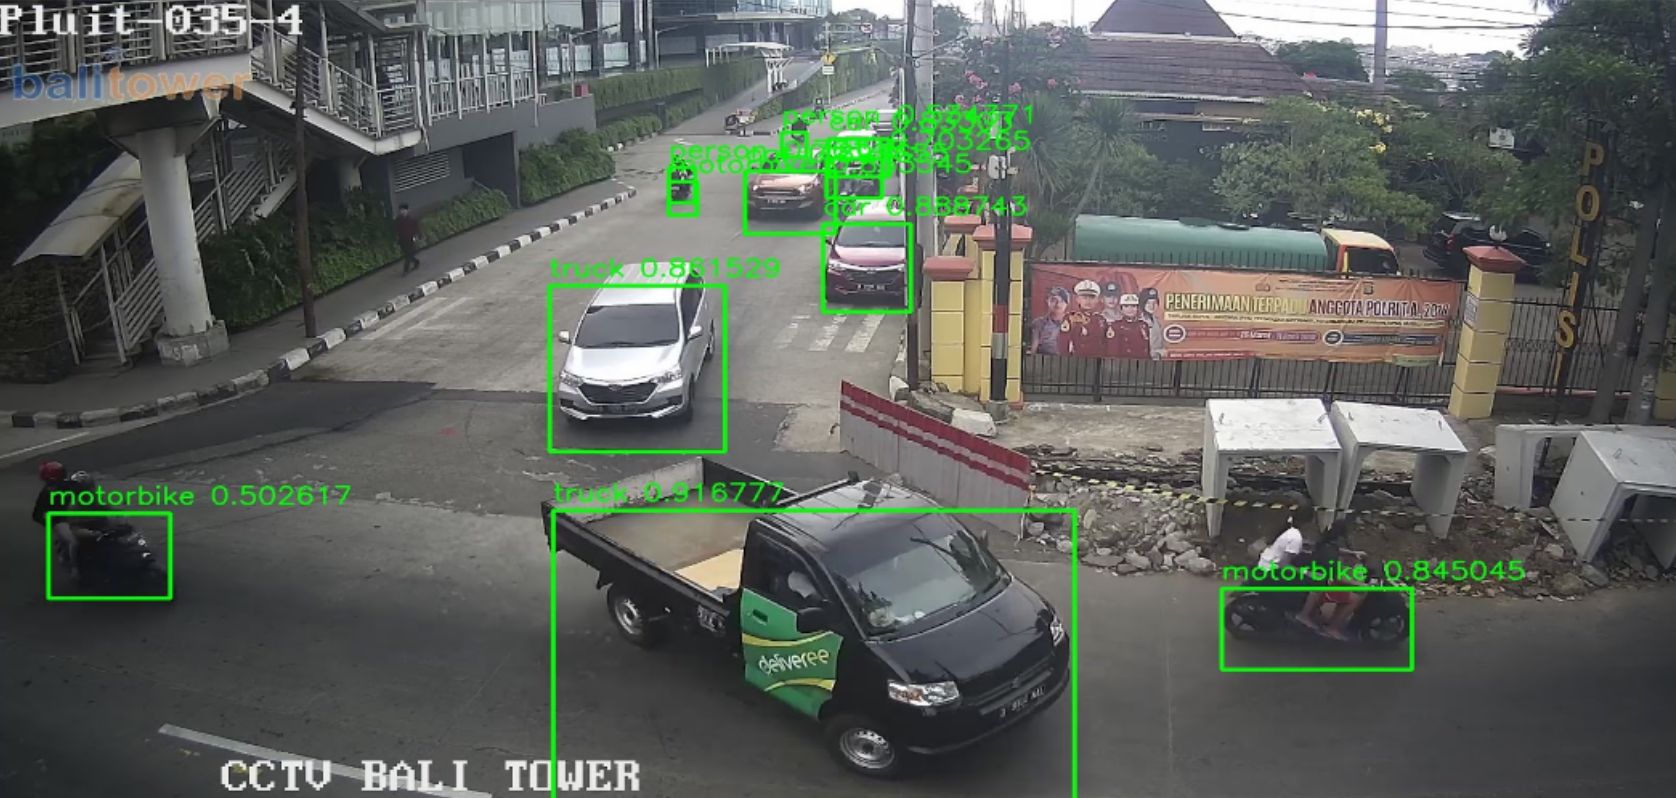
\includegraphics[width=0.9\paperwidth]{figures/jakarta_traffic}
    \caption{Automatically parsing traffic camera images can help with traffic
      management. \label{fig:label} }
  \end{figure}
\end{frame}

\begin{frame}
  \frametitle{Sensing: Conservation through Land Use Maps}
  \begin{figure}[ht]
    \centering
    \includegraphics[width=0.7\paperwidth]{figures/land_cover}
    \caption{Enhanced land use maps let conservation organizations manage
      ecosystems. \label{fig:land_use} }
  \end{figure}
\end{frame}

\begin{frame}
  \frametitle{Acting: White Fly Prediction}
  \begin{figure}[ht]
    \centering
    \includegraphics[width=0.7\paperwidth]{figures/whitefly}
    \caption{Quickly counting white flies on cassava plants helps agricultural
      extension workers protect crops. \label{fig:whitefly} }
  \end{figure}
\end{frame}

\begin{frame}
  \frametitle{Acting: Lead Paint Inspection}
  \begin{figure}[ht]
    \centering
    \includegraphics[width=0.7\paperwidth]{figures/lead}
    \caption{Data on historical inspection results can guide the best places to
      send health inspectors in the future, since it's impossible to reach every
      household all the time.
      \label{fig:lead_paint} }
  \end{figure}
\end{frame}

\begin{frame}
  \frametitle{Augmentation and Amplification}
  \begin{itemize}
  \item Augmentation: AI tools can make people more effective at reasoning about
    problems
    \begin{itemize}
    \item E.g. Vannever Bush's ``As We May Think'' or Michael Jordan's ``The AI
      Revolution hasn't Started Yet''
    \end{itemize}
  \item Amplification: ``what people get out of technology depends on what they
    can do and want to do even without technology''
    \begin{itemize}
    \item Context and intent are crucial
    \end{itemize}
  \item Augmentation and amplification are almost dual to each other
    \begin{itemize}
    \item Ability vs. Motivation to do task
    \end{itemize}
  \end{itemize}
\end{frame}

\begin{frame}
  \frametitle{Mila Projects...}
 \begin{table}[]
   \begin{tabular}{|p{2cm}|p{4cm}|p{4cm}|}
     \hline
     & \textbf{Sensing}                                            & \textbf{Acting}                                                                      \\ \hline
     Augmenting Education       & Are students are keeping up? & Suggesting students to reach out to                                  \\
     Biasly                     & Presence of gender bias across text sources       & Suggesting alternatives, hold people accountable \\ \hline
     BlindTool                  & The space between your ride and the doorstep      & Navigating the space from ride to doorstep             \\ \hline
     Ganify Climate & Environments before and after climate disasters   & ?                           \\ \hline
     RC Mapping          & Presence of flood-related features in Uganda      & Planning evacuation routes \\  \hline
     Sat. Super-Res & Activities visible from space, at daily frequency & ?                                                                  \\ \hline
     Ubenwa & Does a cry sound like asphyxia? & Consult medical expert \\\hline
   \end{tabular}
 \end{table}
\end{frame}

\begin{frame}
  \frametitle{Mila Projects...}
\begin{table}[]
   \begin{tabular}{|p{2cm}|p{4cm}|p{4cm}|}
     \hline
                           & \textbf{Augments}                       & \textbf{Amplifies}                                                         \\\hline
Augmenting Education       & Evaluation of student recall  & Teachers \\\hline
Biasly                     & Critical reading and writing       & Active readers and attentive writers\\\hline
BlindTool                  & Visual navigation      & People with visual-impairments \\\hline
Ganify Climate & Reasoning about climate future   & Climate activist efforts                                                                           \\\hline
RC Mapping          & Map annotation      & Mapathon volunteers \\\hline
Sat. Super-Res & Geographic reasoning & Anyone using satellite imagery                                                                           \\\hline
Ubenwa & Detection of asphyxia & Concerned parents \\\hline
\end{tabular}
\end{table}
\end{frame}

\begin{frame}
  \frametitle{Humanitarian AI}
  Successful application in resource constrained, real-world scenarios will
  require careful thought on classical topics,
  \begin{itemize}
  \item Data or label collection (active learning, HCI)
  \item Scarce labels (GANS, semisupervised learning)
  \item Heterogeneous data sources (metalearning)
  \item Interpretable systems (explainability)
  \item Probabilistically informed actions (bayesian DL)
  \item Resource-limited deployments (model compression)
  \end{itemize}
\end{frame}

\begin{frame}
  \frametitle{Humanitarian AI}
  \begin{itemize}
  \item How can we ensure that AI benefits everyone?
  \item We need the development of AI research and applications to be
    \textit{inclusive}.
  \item Emphasize training, and avoid careless export
  \end{itemize}
\end{frame}

\begin{frame}
  \frametitle{Conclusion}
  \begin{itemize}
  \item My thoughts about Montreal Humanitarian AI are very preliminary...
  \item There are many related projects in Montreal which I haven't had a chance
    to speak about
  \item Stepping back, the questions in this field challenge us to think about
    old problems in new ways
  \item Let me know if you are interested in sharing any work or have any other
    questions about the reading group
  \end{itemize}
\end{frame}

\end{document}
